\documentclass[twoside]{book}

% Packages required by doxygen
\usepackage{fixltx2e}
\usepackage{calc}
\usepackage{doxygen}
\usepackage[export]{adjustbox} % also loads graphicx
\usepackage{graphicx}
\usepackage[utf8]{inputenc}
\usepackage{makeidx}
\usepackage{multicol}
\usepackage{multirow}
\PassOptionsToPackage{warn}{textcomp}
\usepackage{textcomp}
\usepackage[nointegrals]{wasysym}
\usepackage[table]{xcolor}

% Font selection
\usepackage[T1]{fontenc}
\usepackage[scaled=.90]{helvet}
\usepackage{courier}
\usepackage{amssymb}
\usepackage{sectsty}
\renewcommand{\familydefault}{\sfdefault}
\allsectionsfont{%
  \fontseries{bc}\selectfont%
  \color{darkgray}%
}
\renewcommand{\DoxyLabelFont}{%
  \fontseries{bc}\selectfont%
  \color{darkgray}%
}
\newcommand{\+}{\discretionary{\mbox{\scriptsize$\hookleftarrow$}}{}{}}

% Page & text layout
\usepackage{geometry}
\geometry{%
  a4paper,%
  top=2.5cm,%
  bottom=2.5cm,%
  left=2.5cm,%
  right=2.5cm%
}
\tolerance=750
\hfuzz=15pt
\hbadness=750
\setlength{\emergencystretch}{15pt}
\setlength{\parindent}{0cm}
\setlength{\parskip}{3ex plus 2ex minus 2ex}
\makeatletter
\renewcommand{\paragraph}{%
  \@startsection{paragraph}{4}{0ex}{-1.0ex}{1.0ex}{%
    \normalfont\normalsize\bfseries\SS@parafont%
  }%
}
\renewcommand{\subparagraph}{%
  \@startsection{subparagraph}{5}{0ex}{-1.0ex}{1.0ex}{%
    \normalfont\normalsize\bfseries\SS@subparafont%
  }%
}
\makeatother

% Headers & footers
\usepackage{fancyhdr}
\pagestyle{fancyplain}
\fancyhead[LE]{\fancyplain{}{\bfseries\thepage}}
\fancyhead[CE]{\fancyplain{}{}}
\fancyhead[RE]{\fancyplain{}{\bfseries\leftmark}}
\fancyhead[LO]{\fancyplain{}{\bfseries\rightmark}}
\fancyhead[CO]{\fancyplain{}{}}
\fancyhead[RO]{\fancyplain{}{\bfseries\thepage}}
\fancyfoot[LE]{\fancyplain{}{}}
\fancyfoot[CE]{\fancyplain{}{}}
\fancyfoot[RE]{\fancyplain{}{\bfseries\scriptsize Generated by Doxygen }}
\fancyfoot[LO]{\fancyplain{}{\bfseries\scriptsize Generated by Doxygen }}
\fancyfoot[CO]{\fancyplain{}{}}
\fancyfoot[RO]{\fancyplain{}{}}
\renewcommand{\footrulewidth}{0.4pt}
\renewcommand{\chaptermark}[1]{%
  \markboth{#1}{}%
}
\renewcommand{\sectionmark}[1]{%
  \markright{\thesection\ #1}%
}

% Indices & bibliography
\usepackage{natbib}
\usepackage[titles]{tocloft}
\setcounter{tocdepth}{3}
\setcounter{secnumdepth}{5}
\makeindex

% Hyperlinks (required, but should be loaded last)
\usepackage{ifpdf}
\ifpdf
  \usepackage[pdftex,pagebackref=true]{hyperref}
\else
  \usepackage[ps2pdf,pagebackref=true]{hyperref}
\fi
\hypersetup{%
  colorlinks=true,%
  linkcolor=blue,%
  citecolor=blue,%
  unicode%
}

% Custom commands
\newcommand{\clearemptydoublepage}{%
  \newpage{\pagestyle{empty}\cleardoublepage}%
}

\usepackage{caption}
\captionsetup{labelsep=space,justification=centering,font={bf},singlelinecheck=off,skip=4pt,position=top}

%===== C O N T E N T S =====

\begin{document}

% Titlepage & ToC
\hypersetup{pageanchor=false,
             bookmarksnumbered=true,
             pdfencoding=unicode
            }
\pagenumbering{alph}
\begin{titlepage}
\vspace*{7cm}
\begin{center}%
{\Large My Project }\\
\vspace*{1cm}
{\large Generated by Doxygen 1.8.15}\\
\end{center}
\end{titlepage}
\clearemptydoublepage
\pagenumbering{roman}
\tableofcontents
\clearemptydoublepage
\pagenumbering{arabic}
\hypersetup{pageanchor=true}

%--- Begin generated contents ---
\chapter{Hierarchical Index}
\section{Class Hierarchy}
This inheritance list is sorted roughly, but not completely, alphabetically\+:\begin{DoxyCompactList}
\item \contentsline{section}{Customer\+Item}{\pageref{classCustomerItem}}{}
\item \contentsline{section}{Customer\+Order}{\pageref{classCustomerOrder}}{}
\item \contentsline{section}{Item}{\pageref{classItem}}{}
\item \contentsline{section}{Task}{\pageref{classTask}}{}
\item \contentsline{section}{Utilities}{\pageref{classUtilities}}{}
\item vector\begin{DoxyCompactList}
\item \contentsline{section}{Item\+Manager}{\pageref{classItemManager}}{}
\item \contentsline{section}{Order\+Manager}{\pageref{classOrderManager}}{}
\item \contentsline{section}{Task\+Manager}{\pageref{classTaskManager}}{}
\end{DoxyCompactList}
\end{DoxyCompactList}

\chapter{Class Index}
\section{Class List}
Here are the classes, structs, unions and interfaces with brief descriptions\+:\begin{DoxyCompactList}
\item\contentsline{section}{\mbox{\hyperlink{classw8_1_1DataTable}{w8\+::\+Data\+Table$<$ T $>$}} }{\pageref{classw8_1_1DataTable}}{}
\end{DoxyCompactList}

\chapter{Class Documentation}
\hypertarget{classw7_1_1iProduct}{}\section{w7\+:\+:i\+Product Class Reference}
\label{classw7_1_1iProduct}\index{w7\+::i\+Product@{w7\+::i\+Product}}


{\ttfamily \#include $<$i\+Product.\+h$>$}

Inheritance diagram for w7\+:\+:i\+Product\+:\begin{figure}[H]
\begin{center}
\leavevmode
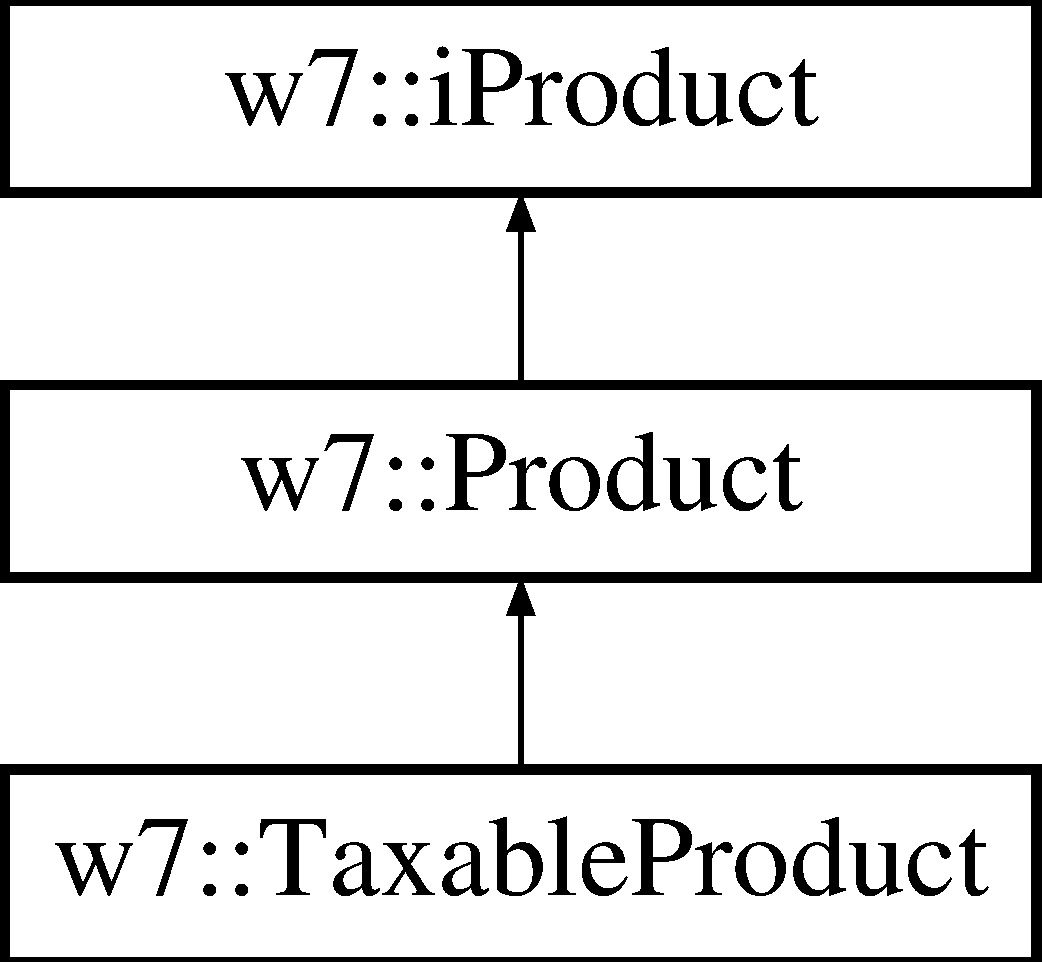
\includegraphics[height=3.000000cm]{classw7_1_1iProduct}
\end{center}
\end{figure}
\subsection*{Public Member Functions}
\begin{DoxyCompactItemize}
\item 
virtual double \mbox{\hyperlink{classw7_1_1iProduct_a4e9fde11cffac0e4309c89d252db89bb}{get\+Charge}} () const =0
\item 
virtual void \mbox{\hyperlink{classw7_1_1iProduct_ad5aa580821cd5cac0acd07841019ed82}{display}} (std\+::ostream \&) const =0
\end{DoxyCompactItemize}


\subsection{Detailed Description}
\mbox{\hyperlink{classw7_1_1iProduct}{i\+Product}} interface for the \mbox{\hyperlink{classw7_1_1Product}{Product}} class to derive from. 

\subsection{Member Function Documentation}
\mbox{\Hypertarget{classw7_1_1iProduct_ad5aa580821cd5cac0acd07841019ed82}\label{classw7_1_1iProduct_ad5aa580821cd5cac0acd07841019ed82}} 
\index{w7\+::i\+Product@{w7\+::i\+Product}!display@{display}}
\index{display@{display}!w7\+::i\+Product@{w7\+::i\+Product}}
\subsubsection{\texorpdfstring{display()}{display()}}
{\footnotesize\ttfamily virtual void w7\+::i\+Product\+::display (\begin{DoxyParamCaption}\item[{std\+::ostream \&}]{ }\end{DoxyParamCaption}) const\hspace{0.3cm}{\ttfamily [pure virtual]}}

Interface query function which outputs the details of the current object to the ostream reference recieved. 

Implemented in \mbox{\hyperlink{classw7_1_1TaxableProduct_a57f8cd41d82054c77a7f7f1cf204cc7d}{w7\+::\+Taxable\+Product}}, and \mbox{\hyperlink{classw7_1_1Product_a60b146f19a712d3eadd1b93a48c54e7d}{w7\+::\+Product}}.

\mbox{\Hypertarget{classw7_1_1iProduct_a4e9fde11cffac0e4309c89d252db89bb}\label{classw7_1_1iProduct_a4e9fde11cffac0e4309c89d252db89bb}} 
\index{w7\+::i\+Product@{w7\+::i\+Product}!get\+Charge@{get\+Charge}}
\index{get\+Charge@{get\+Charge}!w7\+::i\+Product@{w7\+::i\+Product}}
\subsubsection{\texorpdfstring{get\+Charge()}{getCharge()}}
{\footnotesize\ttfamily virtual double w7\+::i\+Product\+::get\+Charge (\begin{DoxyParamCaption}{ }\end{DoxyParamCaption}) const\hspace{0.3cm}{\ttfamily [pure virtual]}}

Interface query function which returns the price of the product. 

Implemented in \mbox{\hyperlink{classw7_1_1TaxableProduct_a3f41864e2a88fa6d847b7fcb704f41f9}{w7\+::\+Taxable\+Product}}, and \mbox{\hyperlink{classw7_1_1Product_a6d73613659451d1492541ef3d0d016b7}{w7\+::\+Product}}.



The documentation for this class was generated from the following file\+:\begin{DoxyCompactItemize}
\item 
i\+Product.\+h\end{DoxyCompactItemize}

\hypertarget{classw7_1_1Product}{}\section{w7\+:\+:Product Class Reference}
\label{classw7_1_1Product}\index{w7\+::\+Product@{w7\+::\+Product}}


{\ttfamily \#include $<$Product.\+h$>$}

Inheritance diagram for w7\+:\+:Product\+:\begin{figure}[H]
\begin{center}
\leavevmode
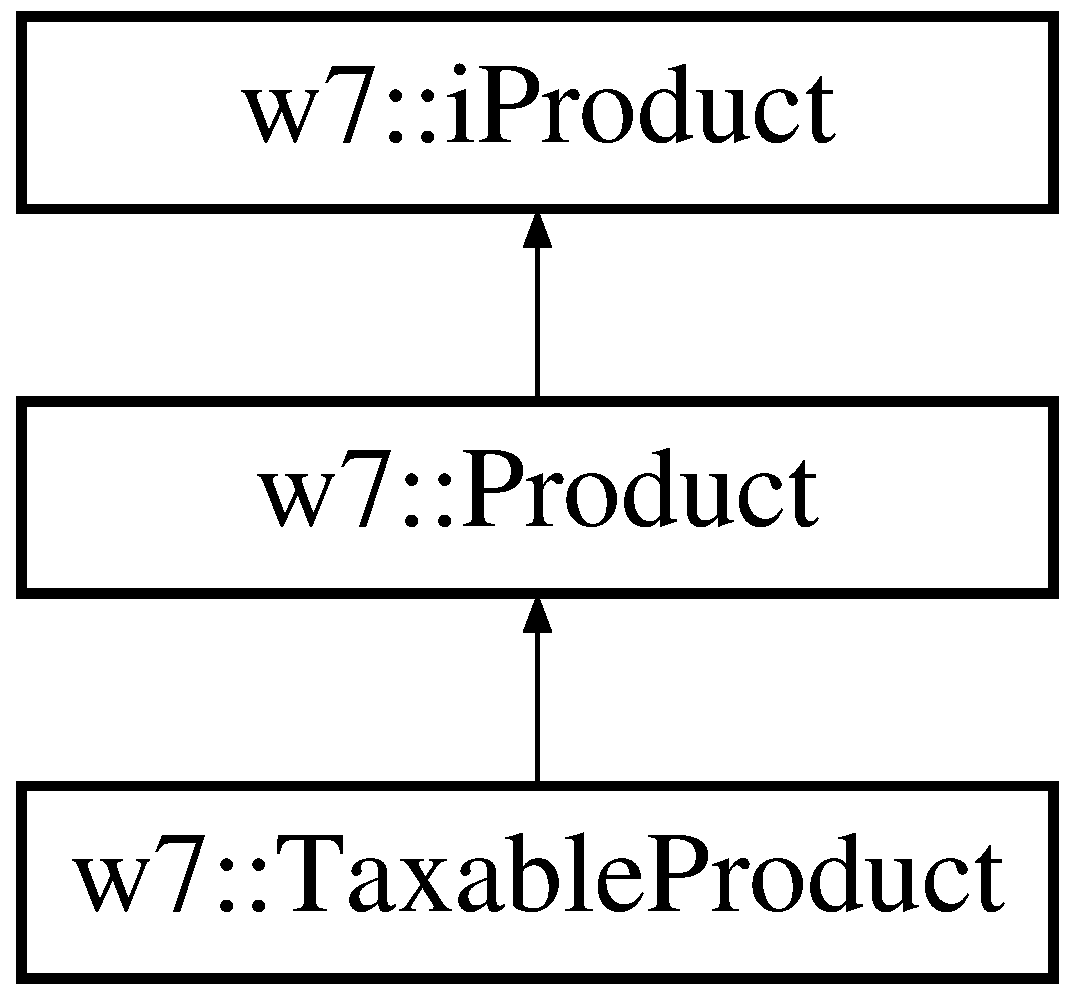
\includegraphics[height=3.000000cm]{classw7_1_1Product}
\end{center}
\end{figure}
\subsection*{Public Member Functions}
\begin{DoxyCompactItemize}
\item 
\mbox{\hyperlink{classw7_1_1Product_a716e2427e981bfd738f6c9c49d0c3ced}{Product}} ()
\item 
\mbox{\hyperlink{classw7_1_1Product_aa5d91c860fae799ab80865c41508fd59}{Product}} (unsigned \+\_\+prod, float \+\_\+cost)
\item 
\mbox{\hyperlink{classw7_1_1Product_adeb7d71bf940bb585977fe07a772190b}{$\sim$\+Product}} ()
\item 
double \mbox{\hyperlink{classw7_1_1Product_a6d73613659451d1492541ef3d0d016b7}{get\+Charge}} () const
\item 
void \mbox{\hyperlink{classw7_1_1Product_a60b146f19a712d3eadd1b93a48c54e7d}{display}} (std\+::ostream \&) const
\end{DoxyCompactItemize}


\subsection{Detailed Description}
\mbox{\hyperlink{classw7_1_1Product}{Product}} class which inherits from \mbox{\hyperlink{classw7_1_1iProduct}{i\+Product}} interface 

\subsection{Constructor \& Destructor Documentation}
\mbox{\Hypertarget{classw7_1_1Product_a716e2427e981bfd738f6c9c49d0c3ced}\label{classw7_1_1Product_a716e2427e981bfd738f6c9c49d0c3ced}} 
\index{w7\+::\+Product@{w7\+::\+Product}!Product@{Product}}
\index{Product@{Product}!w7\+::\+Product@{w7\+::\+Product}}
\subsubsection{\texorpdfstring{Product()}{Product()}\hspace{0.1cm}{\footnotesize\ttfamily [1/2]}}
{\footnotesize\ttfamily w7\+::\+Product\+::\+Product (\begin{DoxyParamCaption}{ }\end{DoxyParamCaption})}

Default constructor that initializes object to an empty state \mbox{\Hypertarget{classw7_1_1Product_aa5d91c860fae799ab80865c41508fd59}\label{classw7_1_1Product_aa5d91c860fae799ab80865c41508fd59}} 
\index{w7\+::\+Product@{w7\+::\+Product}!Product@{Product}}
\index{Product@{Product}!w7\+::\+Product@{w7\+::\+Product}}
\subsubsection{\texorpdfstring{Product()}{Product()}\hspace{0.1cm}{\footnotesize\ttfamily [2/2]}}
{\footnotesize\ttfamily w7\+::\+Product\+::\+Product (\begin{DoxyParamCaption}\item[{unsigned}]{\+\_\+prod,  }\item[{float}]{\+\_\+cost }\end{DoxyParamCaption})}

Constructor which recieves an unsigned integer and float datatype to initialize the object based on the given parameters. \mbox{\Hypertarget{classw7_1_1Product_adeb7d71bf940bb585977fe07a772190b}\label{classw7_1_1Product_adeb7d71bf940bb585977fe07a772190b}} 
\index{w7\+::\+Product@{w7\+::\+Product}!````~Product@{$\sim$\+Product}}
\index{````~Product@{$\sim$\+Product}!w7\+::\+Product@{w7\+::\+Product}}
\subsubsection{\texorpdfstring{$\sim$\+Product()}{~Product()}}
{\footnotesize\ttfamily w7\+::\+Product\+::$\sim$\+Product (\begin{DoxyParamCaption}{ }\end{DoxyParamCaption})}

Default constructor with no dynamic data to handle. 

\subsection{Member Function Documentation}
\mbox{\Hypertarget{classw7_1_1Product_a60b146f19a712d3eadd1b93a48c54e7d}\label{classw7_1_1Product_a60b146f19a712d3eadd1b93a48c54e7d}} 
\index{w7\+::\+Product@{w7\+::\+Product}!display@{display}}
\index{display@{display}!w7\+::\+Product@{w7\+::\+Product}}
\subsubsection{\texorpdfstring{display()}{display()}}
{\footnotesize\ttfamily void w7\+::\+Product\+::display (\begin{DoxyParamCaption}\item[{std\+::ostream \&}]{os }\end{DoxyParamCaption}) const\hspace{0.3cm}{\ttfamily [virtual]}}

Query member function which displays the details of the current object to the ostream object reference recieved. 

Implements \mbox{\hyperlink{classw7_1_1iProduct_ad5aa580821cd5cac0acd07841019ed82}{w7\+::i\+Product}}.



Reimplemented in \mbox{\hyperlink{classw7_1_1TaxableProduct_a57f8cd41d82054c77a7f7f1cf204cc7d}{w7\+::\+Taxable\+Product}}.

\mbox{\Hypertarget{classw7_1_1Product_a6d73613659451d1492541ef3d0d016b7}\label{classw7_1_1Product_a6d73613659451d1492541ef3d0d016b7}} 
\index{w7\+::\+Product@{w7\+::\+Product}!get\+Charge@{get\+Charge}}
\index{get\+Charge@{get\+Charge}!w7\+::\+Product@{w7\+::\+Product}}
\subsubsection{\texorpdfstring{get\+Charge()}{getCharge()}}
{\footnotesize\ttfamily double w7\+::\+Product\+::get\+Charge (\begin{DoxyParamCaption}{ }\end{DoxyParamCaption}) const\hspace{0.3cm}{\ttfamily [virtual]}}

Query member function that returns the cost of the current object. 

Implements \mbox{\hyperlink{classw7_1_1iProduct_a4e9fde11cffac0e4309c89d252db89bb}{w7\+::i\+Product}}.



Reimplemented in \mbox{\hyperlink{classw7_1_1TaxableProduct_a3f41864e2a88fa6d847b7fcb704f41f9}{w7\+::\+Taxable\+Product}}.



The documentation for this class was generated from the following files\+:\begin{DoxyCompactItemize}
\item 
Product.\+h\item 
Product.\+cpp\end{DoxyCompactItemize}

\hypertarget{classw7_1_1Sale}{}\section{w7\+:\+:Sale Class Reference}
\label{classw7_1_1Sale}\index{w7\+::\+Sale@{w7\+::\+Sale}}


{\ttfamily \#include $<$Sale.\+h$>$}

\subsection*{Public Member Functions}
\begin{DoxyCompactItemize}
\item 
\mbox{\Hypertarget{classw7_1_1Sale_a4eda8da6337cf8abc7c01143a1aa825f}\label{classw7_1_1Sale_a4eda8da6337cf8abc7c01143a1aa825f}} 
{\bfseries Sale} (const char $\ast$file)
\item 
\mbox{\Hypertarget{classw7_1_1Sale_abf3135ceeee7067b64450c4d9156a4ec}\label{classw7_1_1Sale_abf3135ceeee7067b64450c4d9156a4ec}} 
void {\bfseries display} (std\+::ostream \&os)
\end{DoxyCompactItemize}


\subsection{Detailed Description}
Class that holds information about a set of products sold to a customer. 

The documentation for this class was generated from the following files\+:\begin{DoxyCompactItemize}
\item 
Sale.\+h\item 
Sale.\+cpp\end{DoxyCompactItemize}

\hypertarget{classw7_1_1TaxableProduct}{}\section{w7\+:\+:Taxable\+Product Class Reference}
\label{classw7_1_1TaxableProduct}\index{w7\+::\+Taxable\+Product@{w7\+::\+Taxable\+Product}}


{\ttfamily \#include $<$Taxable\+Product.\+h$>$}

Inheritance diagram for w7\+:\+:Taxable\+Product\+:\begin{figure}[H]
\begin{center}
\leavevmode
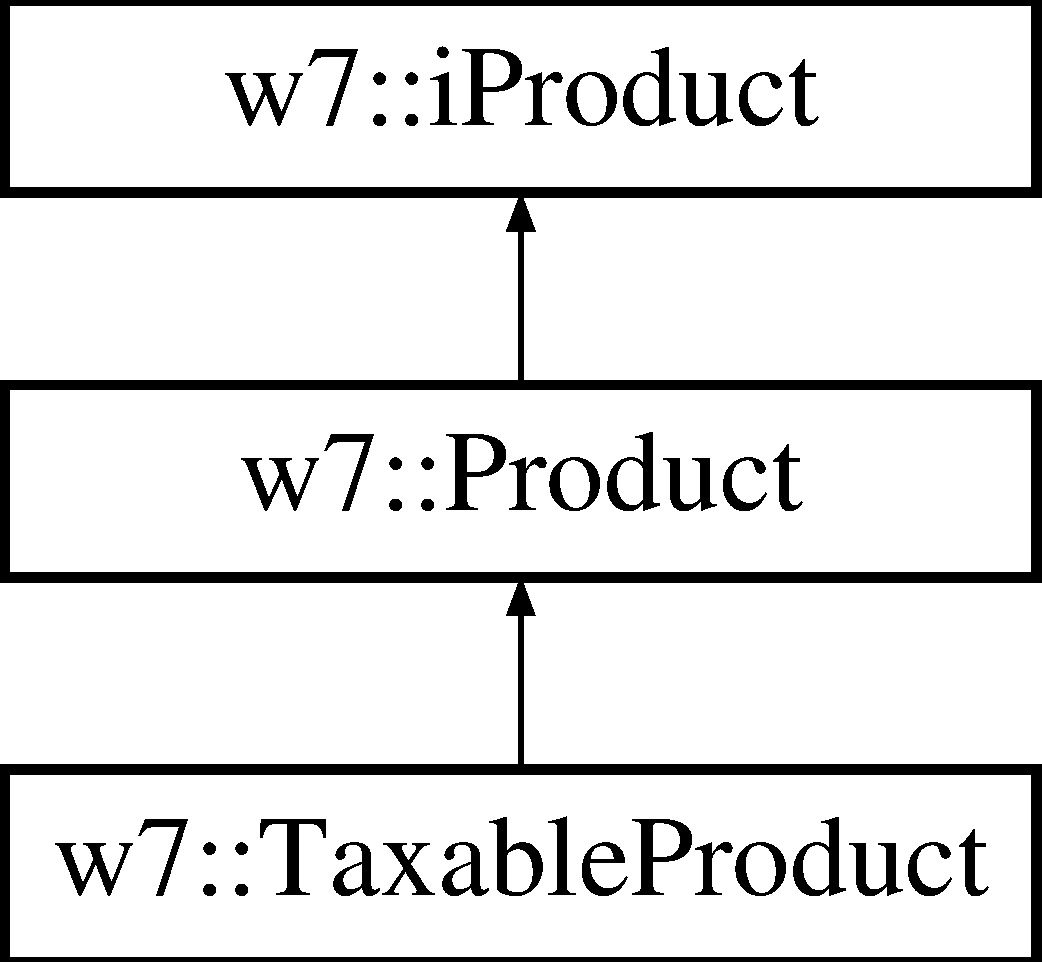
\includegraphics[height=3.000000cm]{classw7_1_1TaxableProduct}
\end{center}
\end{figure}
\subsection*{Public Types}
\begin{DoxyCompactItemize}
\item 
enum \mbox{\hyperlink{classw7_1_1TaxableProduct_a4685ed7e7a83db12a00c004b438e37eb}{Rate}} \{ {\bfseries H}, 
{\bfseries P}
 \}
\end{DoxyCompactItemize}
\subsection*{Public Member Functions}
\begin{DoxyCompactItemize}
\item 
\mbox{\hyperlink{classw7_1_1TaxableProduct_a2e4fb43aefb12ca0778fc4f0a6ffb987}{Taxable\+Product}} (unsigned \+\_\+prod, float \+\_\+cost, char \+\_\+tax\+Status)
\item 
\mbox{\hyperlink{classw7_1_1TaxableProduct_ab9ee3a59e2483d33652ef4103f807e9a}{Taxable\+Product}} ()
\item 
double \mbox{\hyperlink{classw7_1_1TaxableProduct_a3f41864e2a88fa6d847b7fcb704f41f9}{get\+Charge}} () const
\item 
void \mbox{\hyperlink{classw7_1_1TaxableProduct_a57f8cd41d82054c77a7f7f1cf204cc7d}{display}} (std\+::ostream \&) const
\end{DoxyCompactItemize}


\subsection{Detailed Description}
\mbox{\hyperlink{classw7_1_1TaxableProduct}{Taxable\+Product}} object that inherits from the \mbox{\hyperlink{classw7_1_1Product}{Product}} object. 

\subsection{Member Enumeration Documentation}
\mbox{\Hypertarget{classw7_1_1TaxableProduct_a4685ed7e7a83db12a00c004b438e37eb}\label{classw7_1_1TaxableProduct_a4685ed7e7a83db12a00c004b438e37eb}} 
\index{w7\+::\+Taxable\+Product@{w7\+::\+Taxable\+Product}!Rate@{Rate}}
\index{Rate@{Rate}!w7\+::\+Taxable\+Product@{w7\+::\+Taxable\+Product}}
\subsubsection{\texorpdfstring{Rate}{Rate}}
{\footnotesize\ttfamily enum \mbox{\hyperlink{classw7_1_1TaxableProduct_a4685ed7e7a83db12a00c004b438e37eb}{w7\+::\+Taxable\+Product\+::\+Rate}}}

Enumerator to differentiate H\+ST and P\+ST for readability and my own experiment. 

\subsection{Constructor \& Destructor Documentation}
\mbox{\Hypertarget{classw7_1_1TaxableProduct_a2e4fb43aefb12ca0778fc4f0a6ffb987}\label{classw7_1_1TaxableProduct_a2e4fb43aefb12ca0778fc4f0a6ffb987}} 
\index{w7\+::\+Taxable\+Product@{w7\+::\+Taxable\+Product}!Taxable\+Product@{Taxable\+Product}}
\index{Taxable\+Product@{Taxable\+Product}!w7\+::\+Taxable\+Product@{w7\+::\+Taxable\+Product}}
\subsubsection{\texorpdfstring{Taxable\+Product()}{TaxableProduct()}\hspace{0.1cm}{\footnotesize\ttfamily [1/2]}}
{\footnotesize\ttfamily w7\+::\+Taxable\+Product\+::\+Taxable\+Product (\begin{DoxyParamCaption}\item[{unsigned}]{\+\_\+prod,  }\item[{float}]{\+\_\+cost,  }\item[{char}]{\+\_\+tax\+Status }\end{DoxyParamCaption})}

Constructor that initializes the object using a parametered unsigned integer, float datatype, and char datatype. \mbox{\Hypertarget{classw7_1_1TaxableProduct_ab9ee3a59e2483d33652ef4103f807e9a}\label{classw7_1_1TaxableProduct_ab9ee3a59e2483d33652ef4103f807e9a}} 
\index{w7\+::\+Taxable\+Product@{w7\+::\+Taxable\+Product}!Taxable\+Product@{Taxable\+Product}}
\index{Taxable\+Product@{Taxable\+Product}!w7\+::\+Taxable\+Product@{w7\+::\+Taxable\+Product}}
\subsubsection{\texorpdfstring{Taxable\+Product()}{TaxableProduct()}\hspace{0.1cm}{\footnotesize\ttfamily [2/2]}}
{\footnotesize\ttfamily w7\+::\+Taxable\+Product\+::\+Taxable\+Product (\begin{DoxyParamCaption}{ }\end{DoxyParamCaption})}

Default constructor which initializes the object to an empty state. 

\subsection{Member Function Documentation}
\mbox{\Hypertarget{classw7_1_1TaxableProduct_a57f8cd41d82054c77a7f7f1cf204cc7d}\label{classw7_1_1TaxableProduct_a57f8cd41d82054c77a7f7f1cf204cc7d}} 
\index{w7\+::\+Taxable\+Product@{w7\+::\+Taxable\+Product}!display@{display}}
\index{display@{display}!w7\+::\+Taxable\+Product@{w7\+::\+Taxable\+Product}}
\subsubsection{\texorpdfstring{display()}{display()}}
{\footnotesize\ttfamily void w7\+::\+Taxable\+Product\+::display (\begin{DoxyParamCaption}\item[{std\+::ostream \&}]{os }\end{DoxyParamCaption}) const\hspace{0.3cm}{\ttfamily [virtual]}}

Query member function that outputs the object\textquotesingle{}s details to the parametered ostream object reference. 

Reimplemented from \mbox{\hyperlink{classw7_1_1Product_a60b146f19a712d3eadd1b93a48c54e7d}{w7\+::\+Product}}.

\mbox{\Hypertarget{classw7_1_1TaxableProduct_a3f41864e2a88fa6d847b7fcb704f41f9}\label{classw7_1_1TaxableProduct_a3f41864e2a88fa6d847b7fcb704f41f9}} 
\index{w7\+::\+Taxable\+Product@{w7\+::\+Taxable\+Product}!get\+Charge@{get\+Charge}}
\index{get\+Charge@{get\+Charge}!w7\+::\+Taxable\+Product@{w7\+::\+Taxable\+Product}}
\subsubsection{\texorpdfstring{get\+Charge()}{getCharge()}}
{\footnotesize\ttfamily double w7\+::\+Taxable\+Product\+::get\+Charge (\begin{DoxyParamCaption}{ }\end{DoxyParamCaption}) const\hspace{0.3cm}{\ttfamily [virtual]}}

Query member fucntion which returns the charge of the current object multiplied by the type of tax rating. 

Reimplemented from \mbox{\hyperlink{classw7_1_1Product_a6d73613659451d1492541ef3d0d016b7}{w7\+::\+Product}}.



The documentation for this class was generated from the following files\+:\begin{DoxyCompactItemize}
\item 
Taxable\+Product.\+h\item 
Taxable\+Product.\+cpp\end{DoxyCompactItemize}

%--- End generated contents ---

% Index
\backmatter
\newpage
\phantomsection
\clearemptydoublepage
\addcontentsline{toc}{chapter}{Index}
\printindex

\end{document}
